\documentclass{article}
\usepackage{pgf,tikz,tikzscale} 
\usepackage{amssymb}
\usepackage{tcolorbox}
\usepackage{xcolor}
\usepackage[utf8]{inputenc}
\usepackage[english]{babel}
\usepackage{multicol}
\usepackage{enumerate}	
\usepackage{graphicx,lipsum,pgfplots} 
\usepackage{amsmath, amsthm}                 
\usepackage[top=1in,bottom=1in, left=1in, right=1in] {geometry}  
\usepackage{fancyhdr}       
\usepackage{blkarray}


\pagestyle{fancy}              
\lhead{Math 5563 \newline Graph Theory HW2, Ch1}   
\rhead{Warren Keil}







\begin{document}
\setlength{\parindent}{0cm}   %%%%%%%% KEEP THIS  for block style paragraphs. 



%%%%%%%%%%%%%%%%%        1a   %%%%%%%%%%%%%%%%%%%%
\textbf{1.} Is it possible to have a graph \(G\) with degree sequence \((4,3,3,3,2)\)? If not, explain why not.
\vspace{2mm}

\textbf{Solution.} No, it is not possible to have a graph \(G\) to have a degree sequence \((4,3,3,3,2)\). To see why, notice that vertices with odd degree must come in pairs. This is true because every time we add an edge to a graph, then it increase the degree of exactly two vertices by one each. So the first edge will result in the degree sequence having two vertices of odd degree. And since every additional edge will change the parity of precisely two vertices, then the number of vertices with an odd degree will always be an even number.  
\begin{flushright}
\qed
\end{flushright}



\vspace{3mm}
\textbf{2c.} Find a graph in figure 1.9 isomorphic to 

\begin{center}
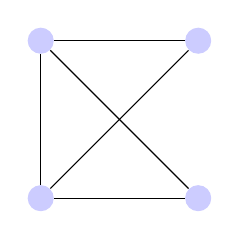
\begin{tikzpicture}
  [scale=.2,auto=left,every node/.style={circle,fill=blue!20}]
  \node (a) at (0,10) {};
  \node (b) at (10,10)  {};
  \node (c) at (10,0)  {};
  \node (d) at (0,0) {};

  \foreach \from/\to in {a/b,a/c,a/d,b/d,c/d}
    \draw (\from) -- (\to);

\end{tikzpicture}.
\end{center}

\textbf{Solution.} The graph from figure 1.9 that is isomorphic to the graph pictured above is the second graph from the left on the bottom row. To prove they are isomorphic, we will arbitrary label the vertices on the graph above and show that an isomorphism exists. The labeling of the vertices are: 

\begin{center}
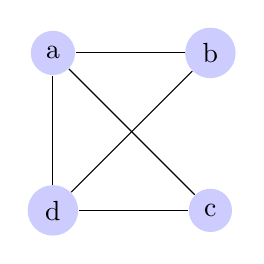
\begin{tikzpicture}
  [scale=.2,auto=left,every node/.style={circle,fill=blue!20}]
  \node (a) at (0,10) {a};
  \node (b) at (10,10)  {b};
  \node (c) at (10,0)  {c};
  \node (d) at (0,0) {d};
  \foreach \from/\to in {a/b,a/c,a/d,b/d,c/d}
    \draw (\from) -- (\to);

\end{tikzpicture} \hspace{20mm} 
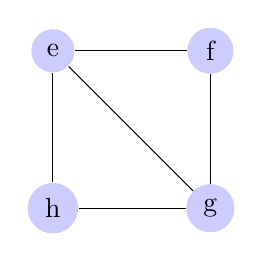
\begin{tikzpicture}
  [scale=.2,auto=left,every node/.style={circle,fill=blue!20}]
  \node (a) at (0,10) {e};
  \node (b) at (10,10)  {f};
  \node (c) at (10,0)  {g};
  \node (d) at (0,0) {h};

  \foreach \from/\to in {a/b,a/c,a/d,b/c,c/d}
    \draw (\from) -- (\to);

\end{tikzpicture}.
\end{center}

Then let the original graph \(G= (V=\{a,b,c,d\}, E=\{ab,ac,ad,bd,cd\} ) \) and the graph from figure 1.9 be \(H = (V'=\{e,f,g,h\}, E'=\{ef,eg,eh,fg,gh,\} )\) . Let \(f:V \rightarrow V' \) such that \(f(a)=e, f(b)=f,\)
\( f(c)=h, f(d)=g\). Then it is easily verified that \(f\) is both one to one and onto. And furthermore, the edge \(ab\) maps to \(f(a)f(b)=ef \), \(ac\) maps to \(f(a)f(c)=eh \), \(ad\) maps to \(f(a)f(d)=eg \), \(bd\) maps to \(f(b)f(d)=fg \), and \(cd\) maps to \(f(c)f(d)=gh \). Thus, \(f\) is an isomorphism and this implies that the two graphs are isomorphic. 
\begin{flushright}
\(\qed\)
\end{flushright}



\vspace{3mm}

\textbf{4b.} Claim: If graph \(G_1\) is isomorphic to graph \(G_2\), then \(G_2\) is isomorphic to \(G_1\). 

\vspace{3mm}  

\textbf{Proof.} Let \(G_1=(V_1,E_1), G_2=(V_2,E_2)\) be graphs such that \(G_1\) is isomorphic to \(G_2\). Then there exists a bijective function \(f:V_1 \rightarrow V_2\) such that for every edge \( uv \in E_1\), the edge \(f(u)f(v)\) is in \( E_2\). To show that \(G_2\) is isomorphic to \(G_1\), we need to show that there exists another bijective function \(g:V_2 \rightarrow V_1\) with the property that an edge \(\hat v \hat u \) is in \(E_2\) if and only if the edge \(g(\hat v)g(\hat u)\) is in \(E_1\). Let \(g:V_2 \rightarrow V_1 : g = f^{-1}\). We know \(f^{-1}\) exists and is a bijective function since \(f\) is a bijection. Let \(uv\) be an edge in \(E_2\). Then this edge is in \(E_2\) if and only if there is an edge \(xy \in E_1\) such that \(uv=f(x)f(y)\). This is true if and only if \( f^{-1}(u)f^{-1}(v)=xy = g(u)g(v)\). And since the edge we picked was arbitrary, then this is true for all edges. Thus, we have shown that an edge \(uv\) is in \( E_2\), if and only if the function \(g=f^{-1}\) maps that edge to an edge \(xy \in E_1\). Therefore, \(g\) is an isomorphism from \(G_1\) to \(G_2\). \(\therefore G_2 \) is isomorphic to \(G_1\). 

\begin{flushright}
\( \blacksquare \) 
\end{flushright}

\newpage

\textbf{4c.} Claim: If \(G_1\) is isomorphic to \(G_2\) and \(G_2\) is isomorphic to \(G_3\), then \(G_1\) is isomorphic to \(G_3\). 

\vspace{3mm}  

\textbf{Proof.} Suppose \(G_1=(V_1,E_1)\) is isomorphic to \(G_2=(E_2,V_2)\) and \(G_2\) is isomorphic to \(G_3=(V_3,E_3)\). Then there exists a bijection \(f:V_1\rightarrow V_2\) such that \(u_1 v_1 \in E_1 \iff f(u_1)f(v_1) \in E_2\). And there exists a bijection \(g:V_2 \rightarrow V_3\) such that \( u_2 v_2 \in E_2 \iff g(u_2)g(v_2) \in E_3\). Let \(h:V_1 \rightarrow V_3 : h = g \circ f \).  The from elementary proofs, we know that \(h\) is a one to one correspondence between \(V_1\) and \(V_3\). To show that \(h\) preserves the edges between \(E_1\) and \(E_3\), let \(u_1 v_1 \in E_1\). We know \(u_1 v_1 \in E_1 \iff f(u_1)f(v_1) \in E_2\). And \( f(u_1)f(v_1) \in E_2 \iff g(f(u_1))g(f(v_1)) \in E_3 \). And since \(h=g\circ f\), then we have shown 
\[
u_1v_1 \in E_1 \iff h(u_1)h(v_1) \in E_3.
\]
\(\therefore G_1\) is isomorphic to \(G_3\).
\begin{flushright}
\( \blacksquare \) 
\end{flushright}



\vspace{3mm}  

\textbf{7.} Let \(G\) be a graph with \(n\) vertices and \(m\) edges. Prove that \(\delta(G) \leq 2m/n\leq \Delta(G) \). 

\vspace{3mm}

\textbf{Proof.} Let \(G\) be a graph with \(n\) vertices and \(m\) edges. First, observe that each edge \(m\) adds two to the total degrees of the vertices. So \(\sum d(v_i) = 2m\). Next, let \( [ d(v_1), d(v_2), \ldots, d(v_n)]\) be the degree sequence of \(G\). Then \(\delta(G)\) is defined as \( \min([ d(v_1), d(v_2), \ldots, d(v_n)]\). Then it is apparent that \(\delta(G)\) is maximized when the degrees of the vertices are spread out as evenly as possible. It follows the \(\delta(G) \leq \lfloor  \frac{2m}n\rfloor  \leq \frac{2m}n\). Next, we notice that \(\Delta(G) \) is minimized when the \(m\) edges are distributed as evenly as possible across the \(n\) vertices. It follows from this that \(\Delta(G)\geq \lceil \frac{2m}n \rceil \geq \frac{2m}n  \). Putting the two parts together, we have shown
\[\delta(G) \leq 2m/n\leq \Delta(G). \] 
\begin{flushright}
\( \blacksquare \) 
\end{flushright}

\vspace{3mm}  

\textbf{20a.} Illustrate the connected antiregular graphs on 5 vertices. 

\vspace{3mm}  

\textit{Solution.} First we construct the possible degree sequences for this antiregular graph to find \(d(G) =[4,3,2,1,4] \) or \( d(V) = [4,3,2,1,2] \). Notice these are only two possible degree sequences since we must have an even number of vertices with odd degree. Next, we notice that for the first degree sequence, however we draw the edges to satisfy the first four degrees \([4,3,2,1]\), since we have a degree of one, then there will be no way to have an additional vertex with degree four. So this leaves the only possible degree sequence of \(d(G) = [4,3,2,1,2,]\). After trial and error, the anitregular graph(s) are/(is): 
\begin{center}
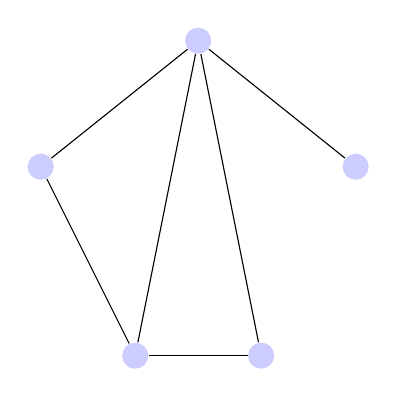
\begin{tikzpicture}
  [scale=.4,auto=left,every node/.style={circle,fill=blue!20}]
  \node (a) at (3,0) {};
  \node (b) at (7,0)  {};
  \node (c) at (0, 6)  {};
  \node (d) at (10,6) {};
  \node (e) at (5,10) {};
  \foreach \from/\to in {e/a,e/b,e/c,e/d,b/a,a/c}
    \draw (\from) -- (\to);

\end{tikzpicture} \hspace{1in}
\begin{tikzpicture}
  [scale=.4,auto=left,every node/.style={circle,fill=blue!20}]
  \node (a) at (3,0) {};
  \node (b) at (7,0)  {};
  \node (c) at (0, 6)  {};
  \node (d) at (10,6) {};
  \node (e) at (5,10) {};
  \foreach \from/\to in {}
    \draw (\from) -- (\to);

\end{tikzpicture}
\end{center}


\newpage

\textbf{20a.} Illustrate the connected antiregular graphs on 6 vertices. 

\vspace{3mm}  

\textit{Solution.} Using the same arguments as above, we come to the conclusion that the only viable degree sequence is \(d(G)=[5,4,3,3,2,1]\). Using brute force, we guess that the unique graph(s) with this degree sequence are/(is): 

\begin{center}
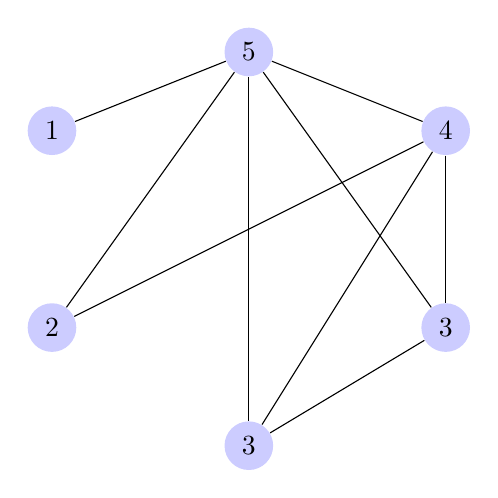
\begin{tikzpicture}
  [scale=.5,auto=left,every node/.style={circle,fill=blue!20}]
  \node (5) at (5,10) {5};
  \node (4) at (10,8)  {4};
  \node (3) at (10, 3)  {3};
  \node (d) at (5,0) {3};
  \node (2) at (0,3) {2};
  \node (1) at (0,8) {1};
  \foreach \from/\to in {5/4,5/3,5/d,5/2,5/1,4/3,4/d,4/2,3/d}
    \draw (\from) -- (\to);

\end{tikzpicture} \hspace{1in}
\begin{tikzpicture}
  [scale=.5,auto=left,every node/.style={circle,fill=blue!20}]
  \node (5) at (5,10) {};
  \node (4) at (10,8)  {};
  \node (3) at (10, 3)  {};
  \node (d) at (5,0) {};
  \node (2) at (0,3) {};
  \node (1) at (0,8) {};
  \foreach \from/\to in {}
    \draw (\from) -- (\to);

\end{tikzpicture}
\end{center}


\vspace{3mm}  

\textbf{25.} For the graphs in Example 1.22, compute \(\det (xI_n - A(G_1))\).

\textit{Solution} Using the mathematica, we use the following code to solve this: 

\begin{verbatim}
Det[{{x, -1, -1, -1}, {-1, x, 0, 0}, {-1, 0, x, -1}, {-1, 0, -1, x}}]
1 - 2 x - 4 x^2 + x^4
\end{verbatim}

This code is interpreted as
 \[ 
\det \left[
\begin{array}{cccc}
 x & -1 & -1 & -1 \\
 -1 & x & 0 & 0 \\
 -1 & 0 & x & -1 \\
 -1 & 0 & -1 & x \\
\end{array}
\right]
=
x^4 -4x^2-2x+1
\]



\end{document}
